%% GTX-GPU technical report -- ACM sigconf layout (same template family as the GTX paper).
%% Build: pdflatex main && bibtex main && pdflatex main && pdflatex main   (or build_paper.bat)
\documentclass[sigconf,nonacm]{acmart}
\settopmatter{printacmref=false, printfolios=true}
\renewcommand\footnotetextcopyrightpermission[1]{}

\usepackage{booktabs}
\usepackage{multirow}
\usepackage{array}
\newcolumntype{P}[1]{>{\raggedright\arraybackslash}p{#1}}
\usepackage{tikz}
\usetikzlibrary{arrows.meta,positioning,calc,shapes.misc,patterns,fit,backgrounds}
\usepackage{pgfplots}
\pgfplotsset{compat=1.18}
\usepgfplotslibrary{groupplots}
\usepackage[ruled,vlined,linesnumbered]{algorithm2e}
\SetAlFnt{\footnotesize}
\SetAlCapFnt{\footnotesize}
\SetAlCapNameFnt{\footnotesize}
\SetCommentSty{textit}

% colours used consistently in every plot
\definecolor{cGTX}{HTML}{1F5FA8}
\definecolor{cCONS}{HTML}{7AA6D6}
\definecolor{cTPL}{HTML}{D95F02}
\definecolor{cSTM}{HTML}{7570B3}
\definecolor{cNOD}{HTML}{1B9E77}
\definecolor{cCAS}{HTML}{8C8C8C}

\newcommand{\sys}{GTX-GPU}
\newcommand{\code}[1]{\texttt{#1}}
\newcommand{\hyp}[1]{\textbf{#1}}

\begin{document}

\title{\sys{}: Latch-free Versioned Graph Transactions with Concurrent Snapshot Readers on GPUs}
\subtitle{Technical Report}

\author{Suyash Kumar}
\email{suyashkumar2005@gmail.com}
\affiliation{%
  \institution{Affiliation}
  \country{Country}}

\begin{abstract}
Dynamic graph structures for GPUs (GPMA, LPMA, Hornet, faimGraph, SlabGraph, Meerkat) sustain hundreds of millions of
edge updates per second, but none of them offers \emph{multi-edge transactions} or \emph{snapshot reads that run
concurrently with updates}. General-purpose GPU software transactional memories provide atomicity, but their conflict
detection is unaware of the graph and collapses under the skew of real-world workloads. This report presents
\sys{}, a GPU adaptation of GTX, a write-optimized latch-free graph transaction system for CPUs. \sys{} keeps GTX's
versioned edge deltas, per-vertex delta blocks, destination-hashed delta chains, lazily resolved transaction
descriptors and epoch-based group commit. It changes four things for the SIMT execution model:
(i)~\emph{destination-precise} write-write conflict detection that validates and CASes on the same observed chain head;
(ii)~\emph{block generations} with lazy chain sealing and a fused generation/fill reservation word, which lets a warp
reserve slots cooperatively and never copies a block under writers;
(iii)~\emph{wait-free epoch registration} with a single advancer lane that publishes a read frontier; and
(iv)~a \emph{serializable} mode that uses Silo-style ordering (epoch fixed before read validation).
Every benchmarked history is validated operation by operation by a checker for snapshot isolation and
serializability, and a paper proof against the PTX memory model covers the protocol. Together they found eight
protocol defects, two of them latent ordering gaps that only the proof could expose.
On an RTX~4060 Laptop GPU, \sys{} is 14--21$\times$ faster than two-phase locking and a TL2 word-STM on the same
storage when 90\% of transactions are snapshot readers. With concurrent readers on Zipf workloads, serializable
read-write mixes on skewed graphs, large transactions or hub contention, the advantage grows to two to four orders of
magnitude. On real SNAP graphs it wins by one to three orders of magnitude where the graph has hubs, and it is
0.66--0.84$\times$ of 2PL where it has none. \sys{} is 6.6--15.2$\times$ faster than GPMA+ on identical streams that
GPMA+ applies correctly. Versions are not reclaimed while a kernel runs, so memory grows with every write. A merge-based
reclamation scheme was built and falsified against criteria fixed in advance. A quiescent compaction between kernel
launches instead keeps memory proportional to the live graph over 64-round update streams, where the uncompacted store runs out
within 1--7 rounds. With the tuned policy it costs 19--30\% of throughput on churn. On a read-heavy stream the
registered policy is 36\% faster. We also report where \sys{} loses: uncontended small
transactions (0.37--0.56$\times$ of 2PL), write-only work against a degree-free STM, and 3--19$\times$ the memory of
pre-sized hash tables.
\end{abstract}

\begin{CCSXML}
<ccs2012>
<concept><concept_id>10002951.10002952.10002953.10010146</concept_id>
<concept_desc>Information systems~Graph-based database models</concept_desc><concept_significance>500</concept_significance></concept>
<concept><concept_id>10002951.10002952.10003190.10003193</concept_id>
<concept_desc>Information systems~Database transaction processing</concept_desc><concept_significance>500</concept_significance></concept>
<concept><concept_id>10010147.10010169.10010170.10010174</concept_id>
<concept_desc>Computing methodologies~Massively parallel algorithms</concept_desc><concept_significance>300</concept_significance></concept>
</ccs2012>
\end{CCSXML}
\ccsdesc[500]{Information systems~Graph-based database models}
\ccsdesc[500]{Information systems~Database transaction processing}
\ccsdesc[300]{Computing methodologies~Massively parallel algorithms}

\keywords{Dynamic graph, GPU, transaction, snapshot isolation, serializability, multi-versioning, latch-free concurrency control}

\maketitle

%% ===================================================================================================================
\section{Introduction}

Dynamic graphs change continuously: edges between users, accounts, devices or road segments are inserted and deleted
while analytics and point queries run over the same graph. GPUs are an attractive home for such graphs. They offer an
order of magnitude more memory bandwidth and thread-level parallelism than a CPU socket, and a line of GPU-resident
dynamic-graph structures has pushed raw update rates into the hundreds of millions of edges per second. SlabGraph, for
example, reports 501--641~MEdge/s for batched insertions on a TITAN~V~\cite{slabgraph}.

These structures share one gap. They apply updates \emph{batch-at-a-time}, with no atomicity across edges and no
consistent view for readers that run while a batch is applied~\cite{gpma,lpma,hornet,faimgraph,slabgraph,meerkat,survey25}.
Applications that must move an edge (delete $(u,v)$, insert $(u,w)$), insert both directions of an undirected edge, or
update an adjacency list together with a degree counter need \emph{multi-edge transactions}. Analytics that run
concurrently with updates need \emph{snapshots}. On the GPU the only general answer today is a software transactional
memory~\cite{gpustm,prstm,csmv}. A word-based STM treats the adjacency structure as anonymous memory words, so every
insert into a hub vertex conflicts on the hub's degree word and on nearby hash slots.

On the CPU, GTX~\cite{gtx} addresses the same problem for main-memory graph systems. It stores each vertex's adjacency
as a block of \emph{edge deltas} (versions with creation and invalidation timestamps). It indexes the deltas by
destination into \emph{delta chains}, which serve both as a lookup accelerator and as the granularity of write-write
conflict detection. Transaction descriptors are resolved lazily by readers, and commit happens in groups against
global read/write epochs. GTX reports up to 11$\times$ higher transaction throughput than LiveGraph, Teseo and
Sortledton on write-heavy, temporally skewed workloads~\cite{gtx,livegraph,teseo,sortledton}.

This report asks whether that architecture can be moved to a GPU, and what must change. Four GPU properties make a
direct port unsuitable:
\begin{itemize}
\item \textbf{Lockstep warps and hub skew.} Thirty-two lanes of a warp often target the same hub vertex. Per-lane
atomics on the vertex's allocation counter serialize at one L2 slice, and blocking locks inside a warp collective can
deadlock.
\item \textbf{No stop-the-world block growth.} GTX consolidates a full edge-delta block by copying it. On a GPU,
thousands of writers may be appending to that block when it fills.
\item \textbf{A weak, scoped memory model.} Every visibility edge (block publication, chain head, descriptor, epoch
frontier) needs an explicit release/acquire argument at device scope. A missing one does not fail loudly; it produces
a rare wrong read.
\item \textbf{Validation at scale.} A kernel commits millions of transactions in milliseconds. Comparing the final graph
against a log, the usual check in GPU prototypes, cannot see lost updates or torn snapshots (\S\ref{sec:checker}).
\end{itemize}

\paragraph{Contributions.}
\begin{enumerate}
\item \textbf{\sys{} design} (\S\ref{sec:arch}--\S\ref{sec:cc}). A GPU-resident multi-version graph store with
transactional edge insertion and deletion, point lookups and adjacency scans, under snapshot isolation (SI) and under
serializability (SER). GTX provides SI only~\cite{gtx}. The GPU-specific mechanisms are destination-precise
validate-then-CAS conflict detection, block generations with lazy sealing, warp-cooperative reservation on a fused
generation/fill word, wait-free epoch registration with a one-lane advancer, and Silo-ordered serializable
validation~\cite{silo}.
\item \textbf{A correctness methodology for GPU transaction protocols} (\S\ref{sec:correct}). Six invariants, a paper
proof of SI and serializability against the PTX memory model with every lemma mapped to a code site and a test, and a
history checker (C1--C5) that validates \emph{every} read, no-op write and scan against its snapshot, write-write
exclusion, the final state and serialization-graph acyclicity. The checker and stress tests found six protocol
defects and the proof two more, and the checker rejects every observable deliberately broken protocol, several of
which pass the final-state check.
\item \textbf{A matched evaluation} (\S\ref{sec:eval}). Same workload streams and seeds against strict two-phase locking,
a TL2-style word STM~\cite{tl2} with and without a degree word, non-transactional CAS updates, and GPMA+~\cite{gpma},
on synthetic streams, four real SNAP graphs and a batch-size sweep. Results are medians of five repetitions with 95\%
bootstrap confidence intervals, and losses are reported next to wins.
\item \textbf{Falsifiable design hypotheses} (\S\ref{sec:ablation}, \S\ref{sec:memory}). Each mechanism was stated with
a falsification criterion before it was measured. Cooperative reservation was falsified as a primary mechanism,
destination-precise conflicts were supported, and epoch commit groups were not falsified. Version reclamation by
generation merging (M4) was built, proven and gated, and then falsified on time and memory.
\item \textbf{Bounded memory by quiescent compaction} (\S\ref{sec:memory}). Memory was measured before any redesign:
most of the overhead is layout, not garbage. Method~5 rebuilds the store from the graph visible at the frontier
between kernel launches. It is proven, gated with mutations, and measured on long update streams that write several
times the arena.
\end{enumerate}

%% ===================================================================================================================
\section{Background and Related Work}
\label{sec:related}

\subsection{GTX}
GTX~\cite{gtx} is a main-memory, latch-free graph data system. Each vertex owns an \emph{edge-delta block}, an
append-only array of edge deltas. A delta records an operation on edge $(u,v)$ together with a creation timestamp and
an invalidation timestamp. A small \emph{delta-chains index} per block hashes destinations to chains. A writer takes
a lock bit in the chain's index entry by CAS and aborts if the CAS fails, a granularity the authors describe as
``a middle ground between vertex and edge locks''. Transactions obtain snapshots from global read/write epochs,
following LiveGraph~\cite{livegraph}. Commit is a hybrid group commit, and timestamps are written into deltas lazily
after commit. GTX supports \emph{snapshot isolation only}: it detects write-write conflicts but not read-write
conflicts.

\subsection{Dynamic graphs on GPUs}
Table~\ref{tab:space} summarizes the design space, following the recent survey of Lin, Zou and Su~\cite{survey25}.
GPMA and GPMA+ keep edges in a sorted packed memory array. GPMA+ replaces GPMA's lock-based segment updates with
lock-free, segment-oriented batch updates and reports up to 18.30$\times$ over GPMA~\cite{gpma,gpmatr}. LPMA levels
the PMA to avoid global reallocation and reports 6--20$\times$ over GPMA+~\cite{lpma}. Hornet~\cite{hornet} and
faimGraph~\cite{faimgraph} manage per-vertex arrays or pages with GPU-side allocators, and faimGraph also reclaims
memory. SlabGraph~\cite{slabgraph} builds per-vertex SlabHash tables~\cite{slabhash} updated by warp-cooperative
lock-free CAS. Meerkat~\cite{meerkat} extends SlabGraph with iterators for dynamic algorithms. All of these optimize
the \emph{throughput of a batch}. None provides transactions spanning several edges or readers that observe a
consistent state while a batch is in flight.

\begin{table}[t]
\caption{Design space of GPU dynamic-graph structures and transactional systems.}
\label{tab:space}
\footnotesize
\setlength{\tabcolsep}{3pt}
\begin{tabular}{@{}>{\raggedright\arraybackslash}p{1.45cm}>{\raggedright\arraybackslash}p{2.2cm}>{\raggedright\arraybackslash}p{2.1cm}>{\raggedright\arraybackslash}p{1.9cm}@{}}
\toprule
System & Representation & Update sync. & Txns / snapshots \\
\midrule
GPMA / GPMA+ & sorted PMA & locks / lock-free segments & none (batch) \\
LPMA & leveled PMA & segment updates & none \\
Hornet & per-vertex arrays & batched & none \\
faimGraph & linked pages + reclaim & warp per list & none \\
SlabGraph, Meerkat & per-vertex slab hash & warp-coop.\ CAS & none \\
GPU STMs & memory words & locks / versions & yes, graph-agnostic \\
GTX (CPU) & delta blocks + chains & latch-free, group commit & SI \\
\textbf{\sys{}} & delta generations + chains & validate-then-CAS, epochs & \textbf{SI and SER} \\
\bottomrule
\end{tabular}
\end{table}

\subsection{Transactional memory on GPUs}
GPU-STM~\cite{gpustm} is a word- and lock-based STM designed around lockstep execution. PR-STM~\cite{prstm} resolves
conflicts with priority rules. CSMV~\cite{csmv} uses a client-server, multi-versioned design. These systems provide
atomic transactions over arbitrary words, but when applied to a graph they see only anonymous words: a degree counter
or an open-addressing probe sequence becomes a conflict hot spot unrelated to the edges a transaction actually
touches. Our STM baseline (\S\ref{sec:setup}) follows TL2~\cite{tl2}, the canonical word-STM design point: a global
version clock, versioned lock records, commit-time sorted locking, and read-only transactions without read sets.

\subsection{Isolation levels}
Snapshot isolation~\cite{berenson} lets a transaction read a consistent snapshot and commit if no concurrent committed
transaction wrote the same items (first-committer-wins). It admits write skew. Serializability forbids it, and a
history is serializable iff its direct serialization graph of ww, wr and rw dependencies is acyclic~\cite{adya}.
Serializable SI~\cite{cahill} and Silo~\cite{silo} add read validation on top of snapshot or optimistic execution.
\sys{} follows Silo's ordering: a writer's commit epoch is fixed \emph{before} its reads are validated.

%% ===================================================================================================================
\section{\sys{} Architecture}
\label{sec:arch}

\sys{} manages a directed graph with a fixed vertex set $V$ entirely in GPU global memory. A single persistent kernel
executes a stream of transactions, each a sequence of $K$ operations drawn from \{\textsc{insert}$(u,v)$,
\textsc{delete}$(u,v)$, \textsc{lookup}$(u,v)$, \textsc{scan}$(u)$\}. Figure~\ref{fig:arch} shows the storage and the
commit machinery. Table~\ref{tab:layout} lists the exact layout.

\begin{figure*}[t]
\centering
\resizebox{\textwidth}{!}{%
\input{arch_fig}}
\caption{\sys{} storage and commit machinery. A vertex's adjacency is a list of block generations, newest first.
Each generation has one chain head per slot, hashed by destination, and a bump-allocated array of 32-byte deltas.
A writer reserves a slot with one RMW on \code{vfill[u]}, validates the chain of its destination and links the delta
by CAS on the chain head it validated. Readers decide visibility through the creator's descriptor and the published
epoch frontier.}
\label{fig:arch}
\end{figure*}

\subsection{Versioned edge deltas}
Every write creates a new \emph{delta} (Table~\ref{tab:layout}), never an in-place update. A delta records its
destination and operation (\textsc{ins}, \textsc{del}, or \textsc{void} for a reserved slot that was never linked),
the index of the previous delta on its chain, the id of the transaction that created it (\code{owner}), its creation
epoch \code{cts} and its invalidation stamp \code{its}. A committed deletion followed by a re-insertion is simply a
newer \textsc{ins} version. The state of an edge for a transaction is the operation of the newest version visible to it.

\begin{table}[t]
\caption{Data layout (all in GPU global memory).}
\label{tab:layout}
\footnotesize
\setlength{\tabcolsep}{3pt}
\begin{tabular}{@{}P{1.55cm}P{6.2cm}@{}}
\toprule
Structure & Contents \\
\midrule
\code{Delta} (32 B) & \code{dstop} (dst:30, op:2), \code{prev}, \code{owner} (txid), \code{cts}, \code{its} (0, \code{TAG|txid}, or epoch); one arena, bump-allocated per block \\
\code{Block} (32 B) & \code{base, cap, nch, chBase, prevGen}; a \emph{generation}; capacity grows by $8\times$ (\code{growShift}~3, default) or $2\times$ \\
heads \code{H[]} & \code{idx:31 | SEAL:1}; \code{nch} $=$ \code{cap/chRatio} heads per generation (default: one per slot) \\
\code{vcur[u]} & current generation, read by readers; published \emph{before} \code{vfill} \\
\code{vfill[u]} (64 b) & \code{(generation<<32) | slots reserved}; writers' reservation word \\
\code{desc[txid]} (64 b) & 0 \textsc{active}, 1 \textsc{aborted}, \code{(e<<2)|2} \textsc{committed} at epoch $e$; fresh per attempt \\
\code{E} (64 b) & \code{(open epoch<<32) | writers registered}; one word $\Rightarrow$ wait-free registration \\
\code{done[2]}, \code{frontier} & completion counters (epoch parity), published read epoch \\
\bottomrule
\end{tabular}
\end{table}

\subsection{Block generations and delta chains}
GTX consolidates a full edge-delta block into a larger one. \sys{} never copies a block while writers are active.
When a vertex's current block fills, exactly one writer (the lane whose reservation lands on slot \code{cap}) allocates
a generation eight times larger (by default; \S\ref{sec:memory} measures $2\times$). The new generation is linked in \emph{front} of the old one through \code{prevGen}
and published by release stores to \code{vcur[u]} and then \code{vfill[u]}. Each generation has its own chain heads,
indexed by a hash of the destination; the default is one head per slot. A chain may therefore continue into older
generations. To keep the order of versions of one key total, the first writer of generation $g{+}1$ that walks an
older generation \emph{seals} that generation's head for its destination (\code{fetch\_or SEAL}) before walking it.
From then on, all installs for that destination go to the newer generation (invariant I2, \S\ref{sec:inv}).

\subsection{Execution model}
The kernel is persistent. Warp~0, lane~0 is the \emph{advancer}, which closes epochs and publishes the read frontier.
Every other lane is a worker that takes transactions from a global counter (one warp-aggregated \code{atomicAdd} per
warp) and runs them to commit, retrying with randomized exponential backoff after an abort. Warps execute
\code{attempt()} collectively, so lanes of one warp share reservation, commit registration and scans. A transaction
gives up after \code{maxAttempts} attempts or on resource exhaustion; give-ups are counted and reported, never hidden.
For each committed transaction the kernel records $(rts, cts, txid, attempts)$ and the result of every operation.
These records feed the history checker.

%% ===================================================================================================================
\section{Transactions and Concurrency Control}
\label{sec:cc}

\subsection{Visibility and operation semantics}
Transaction $T$ begins with snapshot $rts \leftarrow$ \code{frontier} (acquire) and a fresh descriptor in state
\textsc{active}. A version of edge $(u,v)$ is \emph{visible} to $T$ iff $T$ created it, or its creator committed at an
epoch $\le rts$. Visibility is decided by the creator's descriptor (read lazily) or by the stamped \code{cts}. The
state of $(u,v)$ for $T$ is the operation of the newest visible version; an edge with no visible version is absent.

\begin{itemize}
\item \textsc{lookup}$(u,v)$ returns the state, with read-your-writes, and records which delta it observed.
\item \textsc{insert}$(u,v)$ on a present edge (and \textsc{delete} on an absent one) is a \emph{no-op} that behaves as
a read. Otherwise it appends an \textsc{ins} (\textsc{del}) delta. A \textsc{del} also tags the superseded
\textsc{ins} with $\code{its} := \code{TAG}|T$.
\item \textsc{scan}$(u)$ returns every visible \textsc{ins} of $u$ that is not invalidated by a version visible to $T$
(degree and an order-independent hash of the neighbour set).
\item \textsc{abort} publishes \textsc{aborted}. Nothing is rolled back: the aborted deltas are invisible forever.
\end{itemize}

\subsection{Cooperative reservation}
A writer needs one delta slot per effective write. Algorithm~\ref{alg:resv} obtains it. Lanes of a warp that target the
same vertex are grouped with \code{\_\_match\_any\_sync}. The group leader performs one \code{fetch\_add} of the group
size on \code{vfill[u]} and broadcasts the result, and each lane derives its slot from its rank in the group. Because
\code{vfill} packs the generation in its high half, the RMW returns the generation and the slot atomically, and a
lane can never pair a slot index with the wrong block. Only the unique lane that receives slot \code{cap} grows the
vertex. Lanes that overshoot wait (with \code{\_\_nanosleep}) and retry. This wait is bounded by one
\code{allocBlock} under independent thread scheduling. The RMW must be \emph{acq\_rel}: defect D8
(\S\ref{sec:defects}) showed that a relaxed reservation leaves no happens-before edge to the grower's publication
of the new generation.

\begin{algorithm}[t]
\caption{Warp-cooperative slot reservation}
\label{alg:resv}
\KwIn{vertex $u$ for lanes that need a slot}
$grp \leftarrow$ \code{\_\_match\_any\_sync}(FULL, $u$)\;
\If{lane is leader of $grp$}{ $w \leftarrow$ \code{vfill}$[u]$.\code{fetch\_add}(popc($grp$), acq\_rel) }
broadcast $w$; $s \leftarrow \mathrm{low}(w) + \mathrm{rank}(lane, grp)$; $g \leftarrow \mathrm{high}(w)$\;
\uIf{$g = \textsc{none} \wedge s = 0$}{\code{allocBlock}$(u,\textsc{none})$ \tcp*{unique creator}}
\uElseIf{$s < \mathrm{cap}(g)$}{\Return $(g, \mathrm{base}(g)+s)$}
\uElseIf{$s = \mathrm{cap}(g)$}{\code{allocBlock}$(u, g)$ \tcp*{unique grower}}
\Else{wait (\code{\_\_nanosleep}); retry}
\BlankLine
\textbf{allocBlock}$(u, old)$: $B[new] \leftarrow \{base, cap \ll 3, nch, chBase, prevGen{=}old\}$; fence\;
\quad \code{vcur}$[u] \leftarrow new$ (release); \code{vfill}$[u] \leftarrow (new \ll 32)\,|\,0$ (release)\;
\end{algorithm}

\subsection{Destination-precise conflict detection}
GTX detects write-write conflicts at the granularity of a delta chain: a writer aborts if the chain's newest live
delta is not visible to it, whichever destination that delta belongs to. With many destinations hashed onto few
chains and large transactions, most of these aborts are \emph{false}. \sys{} checks only versions of the same
destination (Algorithm~\ref{alg:write}), and it guarantees exclusion by validating and installing against the
\emph{same} observed head $h_0$. If the CAS fails, only the new prefix $h_1 .. h_0$ is walked, and any non-aborted
foreign version of $v$ in it aborts the writer. The walk applies first-updater-wins: an \textsc{active} foreign
version aborts with \code{WW\_PENDING}, and a version committed after $rts$ aborts with \code{WW\_LATE}. The
GTX-faithful rule remains available (\code{dstconf=0}) for ablation and reports its extra aborts as
\code{AB\_CHAIN\_FALSE}.

\begin{algorithm}[t]
\caption{Write (insert/delete) of edge $(u,v)$ by $T$}
\label{alg:write}
$(g, slot) \leftarrow$ \code{reserveSlot}$(u)$\;
$h_0 \leftarrow H[\mathrm{head}(g,v)]$.load(acquire)\;
\lIf{$h_0$.SEAL}{void($slot$); retry reservation}
$r \leftarrow$ \code{walkGens}$(g, h_0, v, \mathit{seal}{=}\mathit{true})$ \tcp*{newest version of $v$}
\ForEach{delta $d$ of $v$ met newest-first}{
  \lIf{$d$.owner $= T$}{found}
  \lElseIf{aborted}{skip}
  \lElseIf{active}{abort(\code{WW\_PENDING})}
  \lElseIf{committed $> rts$}{abort(\code{WW\_LATE})}
  \lElse{found}
}
decide effective / no-op from $r$; on no-op or abort: void($slot$)\;
write delta $\{dstop, prev{=}h_0, owner{=}T\}$\;
\While{$\neg$CAS$(H[\mathrm{head}(g,v)], h_0 \rightarrow slot)$ (acq\_rel)}{
  $h_1 \leftarrow$ observed head\;
  \lIf{$h_1$.SEAL}{void($slot$); retry reservation}
  \lIf{a non-aborted foreign version of $v$ lies in $h_1 .. h_0$}{void($slot$); abort}
  $prev \leftarrow h_1$; $h_0 \leftarrow h_1$\;
}
\lIf{op $=$ DEL}{its(superseded) $\leftarrow$ TAG$|T$}
\end{algorithm}

\subsection{Group commit with epochs}
GTX's group commit uses global read and write epochs. On the GPU, the obvious registration protocol (read \code{E},
increment an in-flight counter, re-read \code{E}, retry on change) \emph{livelocked} for seconds, because the
advancer bumps the epoch about once per microsecond (defect D5). \sys{} makes registration a single RMW
(Algorithm~\ref{alg:commit}). \code{E} packs the open epoch with the number of writers registered in it, so a warp's
leader registers all its committing lanes with one \code{fetch\_add} and receives the epoch in the same instruction.
The advancer closes an epoch with one \code{exchange}, which atomically returns the exact number of registered writers,
waits until \code{done[e\&1]} reaches that count, and only then publishes $\code{frontier} := e$ with a release
store. Readers take snapshots with one acquire load. After commit, lanes lazily stamp \code{cts} on their deltas and
\code{its} on superseded versions, so later readers skip the descriptor lookup.

A transaction that performed no effective write commits at $cts = rts$ without registering. It publishes
\textsc{aborted} rather than \textsc{committed} because it may own reserved-then-voided slots, which must never
become ``committed in the past'' (defect D7).

\begin{algorithm}[t]
\caption{Commit (per warp) and the advancer}
\label{alg:commit}
$W \leftarrow$ lanes alive with $\ge 1$ effective write\;
$e \leftarrow$ \code{E}.\code{fetch\_add}(popc($W$), acq\_rel) $\gg 32$ \tcp*{leader; before validation}
\If{SER}{
  validate point reads: newest non-aborted foreign version of $(u,v)$ is the observed one\;
  validate scans: every foreign non-aborted delta of $u$ visible at $rts$ and not invalidated\;
}
fence; \code{desc}$[T] \leftarrow$ alive ? \textsc{committed}$(e)$ : \textsc{aborted}; \code{\_\_syncwarp}\;
leader: fence; \code{done}$[e \,\&\, 1]$ += popc($W$)\;
stamp: cts(own deltas) $\leftarrow e$; its(superseded) $\leftarrow e$\;
\BlankLine
\textbf{advancer} (one lane)\;
\While{true}{
  $e \leftarrow$ \code{E}.hi; $reg \leftarrow$ \code{E}.\code{exchange}$((e{+}1) \ll 32)$.lo\;
  wait \code{done}$[e\,\&\,1] = reg$; \code{done}$[e\,\&\,1] \leftarrow 0$; \code{frontier} $\leftarrow e$ (release)\;
}
\end{algorithm}

\subsection{Serializable mode}
SI permits write skew. \sys{}'s SER mode adds optimistic read validation at commit. For a point read or a no-op
write, the newest non-aborted foreign version of $(u,v)$ must still be the one observed. For a scan, every foreign,
non-aborted delta of $u$ must be visible at $rts$ and not invalidated by a non-aborted foreign transaction; this is
a predicate (phantom) check. The ordering matters. In our first design the epoch was taken \emph{after} validation,
so an rw anti-dependency $T \rightarrow U$ could run backwards in commit order, and read-only transactions reading
from the frontier saw non-serializable states (defect D6, 5 histories with up to 40,535 serialization-graph back
edges). Fixing the epoch \emph{before} validation (Silo order~\cite{silo}) makes every ww, wr and rw dependency
non-decreasing in commit epoch. A frontier snapshot is then a dependency-closed prefix, and read-only transactions
serialize at $rts$ with no validation at all.

\subsection{Reads and scans}
\textsc{lookup} walks the chain(s) of $v$ from \code{vcur[u]} newest-first and returns the first version visible to
$T$. \textsc{scan} visits every slot $[0, \min(\mathit{fill}, \mathit{cap}))$ of every generation. By default the
whole warp strides one vertex (warp-cooperative scan), which is essential for power-law graphs
(\S\ref{sec:readers}). Readers never write shared state, never wait, and never abort in SI mode.

\subsection{Cost model}
Table~\ref{tab:cost} gives the uncontended cost of one effective write. The dominant fixed cost compared with a
lock-based hash table is versioning: a 32-byte delta, a chain head and descriptor/epoch bookkeeping per attempt.
Scans cost $\Theta$(slots in all generations), including aborted and voided slots, until the next quiescent
compaction rebuilds the store (\S\ref{sec:memory}).

\begin{table}[t]
\caption{Cost per effective write (uncontended).}
\label{tab:cost}
\footnotesize
\setlength{\tabcolsep}{3pt}
\begin{tabular}{@{}P{1.5cm}P{3.7cm}P{2.4cm}@{}}
\toprule
Step & Dependent global round trips & Atomics \\
\midrule
reservation & 1 RMW on \code{vfill[u]} (+1 load of $B[g]$) & 1 per (warp, vertex) \\
walk & 1 + chain length ($\approx$1) + 1 per older gen. & 1 seal per (old gen, chain) \\
install & 1 CAS & 1 \\
commit & 1 RMW on \code{E}, 1 on \code{done} per warp; per lane 1 desc store + stamps & 2 per warp \\
\bottomrule
\end{tabular}
\end{table}

%% ===================================================================================================================
\section{Correctness}
\label{sec:correct}

\subsection{Invariants}
\label{sec:inv}
\begin{description}
\item[I1 Single writer per chain position.] For every key, non-aborted versions are totally ordered by chain
position, and that order equals commit-epoch order. This follows from three rules: an install requires the newest
non-aborted version to be $T$'s own or committed $\le rts$; the CAS is on the same observed head; and a failed CAS
triggers a prefix re-walk.
\item[I2 Generation monotonicity.] If a version of $v$ exists in generation $g{+}1$, the head of $v$'s chain in every
older generation is sealed, so every install into $g$ precedes every install into $g{+}1$ for that key.
\item[I3 Frontier safety.] $\code{frontier} \ge e$ implies that every writer registered in $e$ has published its final
descriptor. Registration and closing are RMWs on one word, and the advancer waits for the exact count.
\item[I4 No torn visibility.] A transaction's versions become visible to a snapshot all-or-nothing, because
visibility depends only on the descriptor or epoch and snapshots cover only completed epochs.
\item[I5 SER ordering.] A writer's epoch is fixed before its validation, so every dependency is non-decreasing in
epoch.
\item[I6 Slot publication.] Every reserved slot is written exactly once by its reserver (content, or \textsc{void}),
and a slot is linked into a chain at most once.
\end{description}

\paragraph{Memory-order requirements.} Each of the following was shown necessary either by a failure or by the
memory model. (1) The grower's stores $B[new] \rightarrow \code{vcur} \rightarrow \code{vfill}$ are releases, and the
reservation \code{fetch\_add} is acq\_rel. (2) The delta contents reach the chain head through an acq\_rel CAS, whose
release sequence covers later readers. (3) Relaxed loads of delta contents suffice for scanners, because a scanner
uses a delta only after establishing its creator's visibility through \code{desc} or \code{frontier} (acquire).
(4) Commit publication is: fence; relaxed descriptor store; \code{\_\_syncwarp}; leader fence; RMW on \code{done};
acquire load by the advancer; release store of the frontier.

\paragraph{Progress.} Writers are lock-free per operation, since a CAS failure implies another install succeeded.
Aborts are no-wait (first-updater-wins). Livelock under identical-edge contention is possible in principle and is
mitigated by randomized exponential backoff. Commit registration is wait-free. The advancer waits only for registered
committers, so in SER mode the frontier's staleness is bounded by the longest validation.

\subsection{Paper proof}
\label{sec:proof}
The repository contains a hand proof (\code{design/proof.md}) that every history of the engine satisfies SI in SI mode
and serializability in SER mode, against the PTX memory model. It is not machine-checked. It assumes device-scope
atomics, ordering only from \code{\_\_syncwarp} and fences (never from warp votes or shuffles, which the CUDA guide
states imply no memory ordering), no slot or descriptor reuse within a kernel run, and quiescence between launches.
Five lemmas on descriptors and epochs (finality, exact registration, frontier safety, fresh epochs, a stable
visible/invisible split) give Theorem~1 (a total per-key version order equal to commit order), Theorem~2 (reads and
no-op writes return the snapshot state), Theorem~3 (scans), Theorem~4 (SI) and Theorem~5 (SER, via Silo ordering).
Section~8 of the proof extends it to the M4 reclamation machinery and \S9 to quiescent compaction (Theorem~6,
\S\ref{sec:memory}). Each lemma names the code site it depends on and the test or mutation that exercises it.

Writing the proof found two latent ordering gaps that no test had observed (D11, D12 in Table~\ref{tab:defects}).
Commit registration ordered the lanes of a warp only through \code{\_\_ballot\_sync}/\code{\_\_shfl\_sync}, and in
cooperative scans every lane loaded the generation list itself although only one lane held the frontier acquire.
Both are fixed (\code{\_\_syncwarp} around registration; the scanning lane reads the generation list and broadcasts
it), at a cost of at most 1\%.

The proof covers every combination of SER/SI, cooperative reservation, conflict granularity, scan mode and pre-walk
for the base protocol. One M4 mutation (per-lane generation lists in cooperative scans) is not observable on this GPU
because of SIMT lockstep. It is covered by the proof alone.

\subsection{History checker}
\label{sec:checker}
A final-state comparison (``the logged edge set equals the device's edge set'') cannot detect a lost update between two
deletions, a torn snapshot, or a dirty read that is later overwritten. Our audit of an earlier GPU prototype found all
three, and each passed that check. \sys{} is instead validated by a host-side checker over the full history. Let
$S(e)$ be the graph after applying, in $cts$ order, the net writes of all committed transactions with $cts \le e$.
\begin{description}
\item[C1 Read rule.] Every read, no-op write and scan result equals $S(rts)$ overlaid with $T$'s own earlier writes;
effective writes agree with the same state.
\item[C2 Observation identity.] A point read names exactly the delta the rule predicts, never an aborted or
uncommitted one.
\item[C3 Write-write.] No committed writer of key $k$ has $cts \in (rts(T), cts(T))$ for another writer $T$ of $k$,
and no two writers of $k$ share a commit timestamp.
\item[C4 Final state.] The device's final edge set equals $S(\infty)$.
\item[C5 Serialization graph] (SER). The direct serialization graph (ww, wr, rw edges; per-key version order $=$ cts
order; a scan reads every key of its vertex) is acyclic.
\end{description}

\paragraph{Test suite.} Six adversarial workloads (mixed uniform on 256 vertices, 50\% hub mixed, 8 identical hot
edges, delete/re-insert churn on 64 vertices with $K{=}8$, 30\% hub with $K{=}32$, Zipf with 50\% readers) run in eight
configurations spanning SI/SER, cooperative reservation on/off, destination/chain conflict granularity, and
per-lane/cooperative scans. All 48 histories pass C1--C5. A \emph{write-skew probe} must show the anomaly under SI
and must not show it under SER: SI produced 16,000 serialization-graph back edges, SER produced 0, and both pass their
respective checks. A tiny-arena test forces resource exhaustion; the committed prefix remains consistent at every arena
size. The full gate has nine sections (A--I): the base suite, the probe, mutations, exhaustion, the optimistic
pre-walk, M4 histories and mutations, exhaustion under reuse, and M5 multi-round compaction
(\S\ref{sec:memory}). It runs 219 cases (110 of them in section I) with 0 unexpected results (\code{results/m5/gate\_full.txt}). In the 2026-11 campaign, 50 further
history-checked runs cover every benchmarked system, the bulk loader, batch mode and the SNAP file path. All pass,
and so do all baselines in SER mode.

\paragraph{Mutation testing.} To show the checker is sensitive, three broken protocols are compiled in
(Table~\ref{tab:mut}). The checker rejects all three. The prototype-style final-state check accepts two of them.
Further mutations target M4 (four of five observable, all four rejected) and M5 (three rejected, one informational;
\S\ref{sec:memory}).

\begin{table}[t]
\caption{Mutation tests: violations reported by each check (2026-11 gate).}
\label{tab:mut}
\footnotesize
\setlength{\tabcolsep}{2.5pt}
\begin{tabular}{@{}lP{1.45cm}P{4.3cm}@{}}
\toprule
Mutation & Final-state check & History checker \\
\midrule
no ww check & passes (0/0) & 4,186 C3; 10,379 same-epoch writers; 10,137 extra final edges; 7,055 DSG back edges \\
ignore snapshot & passes (0/0) & 9,717 wrong reads; 5,721 wrong scans; 309,371 DSG back edges \\
dirty reads & 944/324 & 10,670 wrong reads; 7,168 wrong scans; 302,858 DSG back edges \\
\bottomrule
\end{tabular}
\end{table}

\subsection{Defects found during development}
\label{sec:defects}
Table~\ref{tab:defects} lists the protocol defects found by the checker, by stress tests, by memory-model reasoning
or by the proof. D5--D9 were found and fixed before the first benchmark was recorded. D10 is in the M4 reclamation code
(off by default) and was found by its gate. D11 and D12 were found by the proof and never observed; they were fixed
before the 2026-11 campaign. D9 teaches a general lesson: a diagnostic mechanism (a watchdog) must never trade safety
for liveness.

\begin{table*}[t]
\caption{Protocol defects found and fixed.}
\label{tab:defects}
\footnotesize
\begin{tabular}{@{}lP{2.6cm}P{4.3cm}P{4.2cm}P{3.5cm}@{}}
\toprule
Id & Detected by & Root cause & Fix & Evidence after fix \\
\midrule
D5 & 180-rep stress + watchdog & register by read-increment-reread of \code{E}; advancer bumps \code{E} $\approx$1/\textmu s $\Rightarrow$ committer starves (1.5--20 s kernels) & wait-free registration: one \code{fetch\_add} on \code{(epoch<<32|count)}; close by \code{exchange} & 180/180 reps in 0.15--1.0 ms \\
D6 & checker C5 & epoch fixed after read validation; rw edge runs backwards in commit order (1--40,535 back edges) & Silo order: register epoch before validation & 0 cycles in all SER histories \\
D7 & reasoning (C1 risk) & read-only commit at $cts{=}rts$ would expose voided slots as committed in the past & read-only commit publishes \textsc{aborted} & suite and check matrix pass \\
D8 & forensic scan instrumentation & relaxed reservation RMW: no happens-before to the grower's generation publication & reservation RMW acq\_rel & memory-order argument; suite pass \\
D9 & checker C1 + decision codes & harness watchdog left the advancer's wait after 20 s and published the frontier early & watchdog only flags; run declared invalid; publishing stops & 4/4 stress iterations and 48 histories pass \\
D10 & M4 gate (abort statistics) & reclaimer zeroed only \code{owner}/\code{dstop} of freed slots; a stale nonzero \code{cts} decided visibility for a reused slot & zero all 32 bytes of every freed delta & gate A--H as expected; proof L14 \\
D11 & proof (latent) & commit registration ordered lanes only by \code{\_\_ballot\_sync}/\code{\_\_shfl\_sync}, which imply no memory ordering & \code{\_\_syncwarp} before and after the registration RMW & gate 67/67; cost within noise \\
D12 & proof review (latent) & in cooperative scans each lane loaded the generation list; only the scanning lane holds the frontier acquire & scanning lane reads the list and broadcasts it & gate 67/67; mutation not observable (proof only) \\
\bottomrule
\end{tabular}
\end{table*}

%% ===================================================================================================================
\section{Evaluation}
\label{sec:eval}

\subsection{Setup}
\label{sec:setup}
\paragraph{Platform.} NVIDIA RTX~4060 Laptop GPU (Ada, sm\_89, 24 SMs, 8~GB, WDDM), CUDA~12.8, Windows~11, compiled
with \code{nvcc -O3 -arch=sm\_89}.

\paragraph{Systems.} All transactional baselines share one storage layout: per-vertex open-addressing hash adjacency
plus a per-vertex degree word, pre-sized from the workload so that, unlike \sys{}, they never pay for growth.
\begin{itemize}
\item \textbf{2PL}: strict two-phase locking with per-vertex reader-writer spinlocks acquired in sorted vertex order
(deadlock-free).
\item \textbf{TL2 STM}: word-based TL2-style STM~\cite{tl2} (global version clock, versioned lock records, lazy write
buffering, commit-time sorted locking, read-set validation; read-only transactions without read sets).
\item \textbf{TL2 STM, no degree}: the same without the degree word. It avoids the hub hot spot but cannot answer
degree queries transactionally.
\item \textbf{Non-transactional CAS}: SlabGraph/faimGraph-style lock-free updates. It provides no atomicity or
snapshots and serves as a lower bound on synchronization cost.
\item \textbf{GTX-conservative}: \sys{} with per-lane reservation and GTX's chain-granularity conflicts, i.e.\ the
closest port of GTX.
\item \textbf{GPMA+}~\cite{gpma}: the authors' implementation, both a Windows port and the pristine upstream build
(within 2\% of each other).
\end{itemize}

\paragraph{Workloads.} A deterministic generator (splitmix64, seed 1) produces one stream that every system consumes.
$|V| = 2^{20}$, the initial graph has 4M edges, and each run has about 1M operations
($2^{20}/K$ transactions of $K$ operations, or $2^{18}$ transactions with $K{=}4$). Sources are uniform, hub
(a fraction of operations on one vertex), Zipf($s{=}1$) or R-MAT. Mixes include inserts, deletes, churn
(50/50 insert/delete), reads, identical-edge contention, and 50\% or 90\% read-only transactions with 10\% scans.
Real graphs (\S\ref{sec:snap}) are four SNAP graphs replayed as sliding-window streams. Long-run memory experiments
(\S\ref{sec:memory}) replay a stream in rounds of $2^{18}$ transactions, one kernel launch per round.

\paragraph{Methodology.} We time the single transactional kernel with CUDA events; initial loading and checking are
excluded. Each (scenario, system) runs in its own process with one warm-up and five measured repetitions, and a 90~s
timeout is recorded as DNF. We report committed transactions/s and \emph{effective} edge changes/s (never attempted
operations). Speedup is the ratio of median committed throughput, with a 95\% bootstrap confidence interval over
repetitions. Latency is measured per transaction with \code{\%globaltimer} from the first attempt to commit, including
retries.

\paragraph{Two campaigns.} All numbers in this section come from the 2026-11 campaign, measured with the final
binaries in one session, unless marked otherwise. Every kernel ran 1.4--2.7$\times$ faster in
2026-11 than in an earlier 2026-09 campaign. The September source rebuilt with the November compiler times
identically, so the shift is not caused by the code or the compiler. Its system-side cause (driver version,
power/clock state) was not isolated. Absolute numbers from the two campaigns are therefore never mixed, and every ratio is
taken within one campaign. Ratios also moved between campaigns (for example, 14.0$\times$ to 19.9$\times$ against 2PL
with 90\% readers), so the 2026-09 ratios are not reused here.

\subsection{Update throughput and transaction size}
Figures~\ref{fig:ksweep-u} and~\ref{fig:ksweep-h} vary the transaction size $K$ for insert-only workloads. On
\emph{uniform} sources (Figure~\ref{fig:ksweep-u}), conflicts are rare and uncontended vertex locks are cheap, so 2PL is
1.8--2.0$\times$ faster than \sys{} up to $K{=}8$. That gap is the fixed cost of the transaction machinery
(\S\ref{sec:losses}). As $K$ grows, lock and read-set footprints grow with it. At $K{=}32$, \sys{} sustains 224~M
effective edges/s while 2PL drops to 211~M ($1.06\times$), TL2 to 2.6~M ($85\times$), and the conservative GTX port to
134~M, because its chain-granularity rule aborts 42\% of attempts.

With a \emph{hub} receiving 50\% of operations (Figure~\ref{fig:ksweep-h}), 2PL does not finish any $K$ within 90~s, and
TL2 collapses to 0.016--3.2~M edges/s with abort ratios above 99.6\% because every insert conflicts on the hub's degree
word. \sys{} stays at 123--204~M edges/s. Only the degree-free STM is competitive at small $K$: it is faster than \sys{}
up to $K{=}4$ (\sys{} reaches 0.64--0.74$\times$ of it) and level at $K{=}8$. At $K{=}32$ it aborts 88\% of attempts
and \sys{} is $3.2\times$ faster.


\begin{figure}[t]
\centering
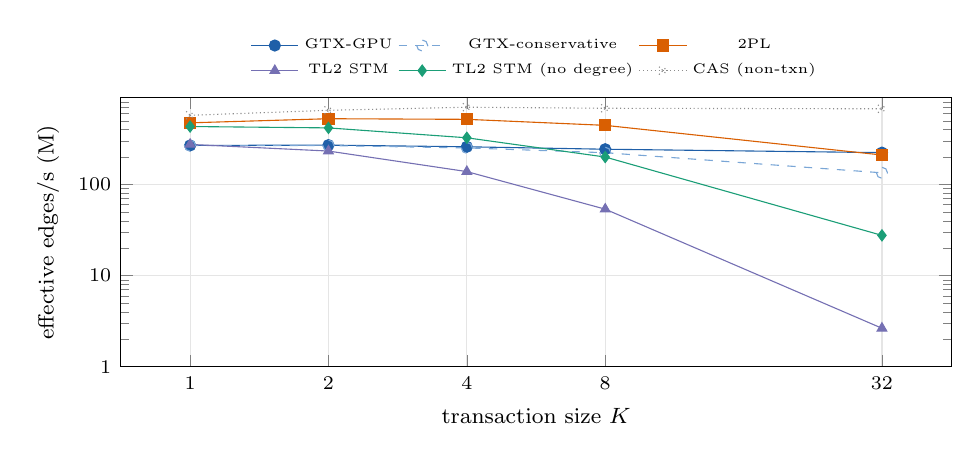
\begin{tikzpicture}
\begin{axis}[width=\columnwidth, height=5.0cm,
    xmode=log, log basis x=2, xtick={1,2,4,8,32}, xticklabels={1,2,4,8,32},
    ymode=log, grid=major, grid style={black!10},
    xlabel={transaction size $K$}, ylabel={effective edges/s (M)},
    tick label style={font=\scriptsize}, label style={font=\footnotesize},
    legend style={font=\tiny, at={(0.5,1.03)}, anchor=south, legend columns=3, draw=none, fill=none}, ymin=1, ymax=900,
    ytick={1,10,100,1000}, yticklabels={1,10,100,1000}]
\addplot[cGTX, mark=*] coordinates {(1,268.6)(2,270.8)(4,259.6)(8,244.1)(32,224.0)}; \addlegendentry{\sys{}}
\addplot[cCONS, mark=o, dashed] coordinates {(1,267.1)(2,267.7)(4,252.4)(8,223.5)(32,134.5)}; \addlegendentry{GTX-conservative}
\addplot[cTPL, mark=square*] coordinates {(1,475.6)(2,527.6)(4,519.5)(8,446.2)(32,210.9)}; \addlegendentry{2PL}
\addplot[cSTM, mark=triangle*] coordinates {(1,275.6)(2,233.1)(4,138.7)(8,53.67)(32,2.646)}; \addlegendentry{TL2 STM}
\addplot[cNOD, mark=diamond*] coordinates {(1,433.3)(2,418.5)(4,325.9)(8,200.4)(32,27.67)}; \addlegendentry{TL2 STM (no degree)}
\addplot[cCAS, mark=x, densely dotted] coordinates {(1,575.3)(2,652.6)(4,705.7)(8,687.2)(32,678.1)}; \addlegendentry{CAS (non-txn)}
\end{axis}
\end{tikzpicture}
\caption{Uniform inserts: effective edge insertions per second vs.\ transaction size ($|V|{=}2^{20}$, 4M initial edges,
1M operations).}
\label{fig:ksweep-u}
\end{figure}

\begin{figure}[t]
\centering
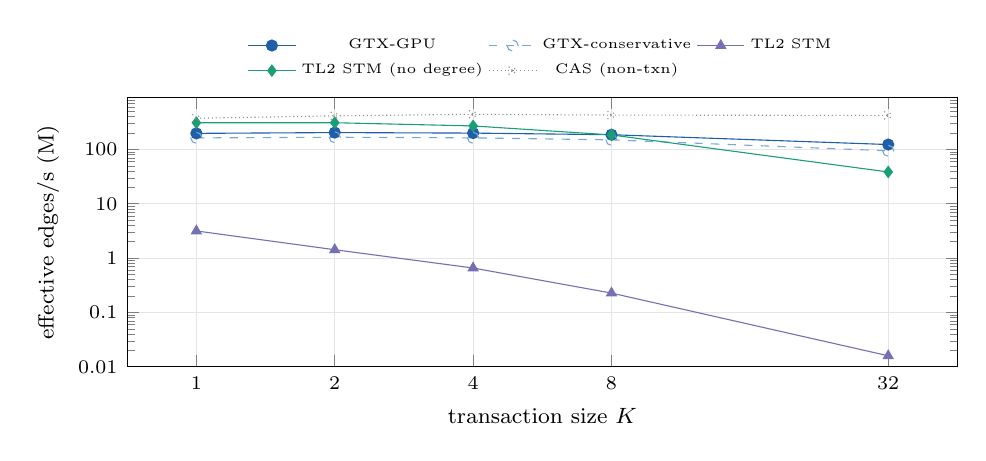
\begin{tikzpicture}
\begin{axis}[width=\columnwidth, height=5.0cm,
    xmode=log, log basis x=2, xtick={1,2,4,8,32}, xticklabels={1,2,4,8,32},
    ymode=log, grid=major, grid style={black!10},
    xlabel={transaction size $K$}, ylabel={effective edges/s (M)},
    tick label style={font=\scriptsize}, label style={font=\footnotesize},
    legend style={font=\tiny, at={(0.5,1.03)}, anchor=south, legend columns=3, draw=none, fill=none}, ymin=0.01, ymax=900,
    ytick={0.01,0.1,1,10,100,1000}, yticklabels={0.01,0.1,1,10,100,1000}]
\addplot[cGTX, mark=*] coordinates {(1,197.7)(2,204.3)(4,199.9)(8,186.7)(32,123.1)}; \addlegendentry{\sys{}}
\addplot[cCONS, mark=o, dashed] coordinates {(1,163.1)(2,167.7)(4,163.4)(8,150.1)(32,94.39)}; \addlegendentry{GTX-conservative}
\addplot[cSTM, mark=triangle*] coordinates {(1,3.161)(2,1.427)(4,0.657)(8,0.2272)(32,0.01593)}; \addlegendentry{TL2 STM}
\addplot[cNOD, mark=diamond*] coordinates {(1,310.2)(2,310.3)(4,270.8)(8,185.0)(32,38.49)}; \addlegendentry{TL2 STM (no degree)}
\addplot[cCAS, mark=x, densely dotted] coordinates {(1,375.4)(2,415.4)(4,443.5)(8,428.7)(32,422.6)}; \addlegendentry{CAS (non-txn)}
\end{axis}
\end{tikzpicture}
\caption{50\% hub inserts. 2PL did not finish any $K$ within 90~s (lower-bound speedups of \sys{}:
$>$18,900$\times$).}
\label{fig:ksweep-h}
\end{figure}

\subsection{Contention, skew and headline comparison}
Figure~\ref{fig:headline} summarizes \sys{}'s speedup over each transactional baseline across the scenarios where
synchronization is hard, together with the uncontended $K{=}1$ case for reference. On power-law churn
(insert/delete mixes, $K{=}4$), 2PL serializes on hub locks: \sys{} is 463$\times$ faster on R-MAT, and 2PL does
not finish on Zipf. TL2 is 96--706$\times$ slower. The degree-free STM beats \sys{} in write-only churn (\sys{} reaches
0.72--0.73$\times$ of it) and in serializable read-write mixes (0.64--0.75$\times$). It loses once scanning readers or
large transactions appear.

Under \emph{identical-edge contention} (50\% of operations on 64 or 1,024 hot edges), every system is dominated by
true conflicts. \sys{} is still 4.0--9.8$\times$ faster than the transactional baselines, because
first-updater-wins with no-wait aborts and backoff wastes less work than lock waits or commit-time validation
failures.

\begin{figure*}[t]
\centering
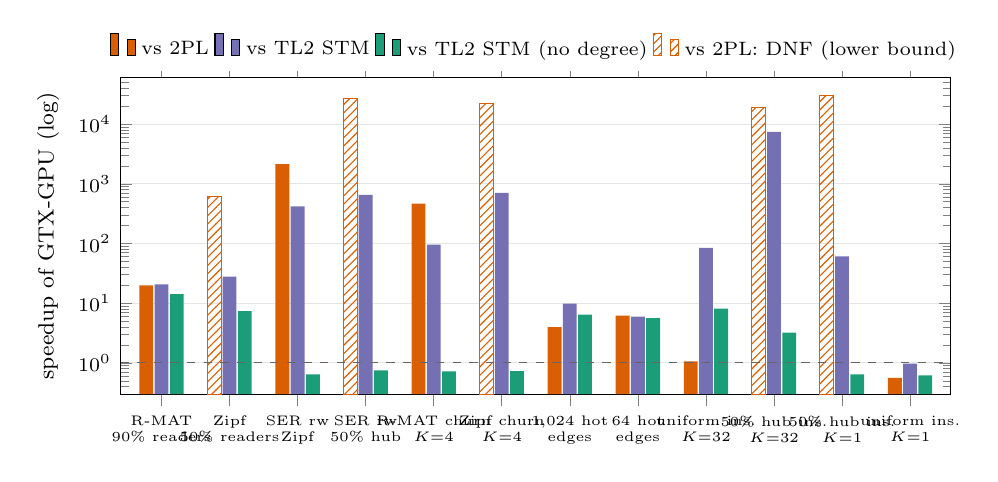
\begin{tikzpicture}
\begin{axis}[
  width=\textwidth, height=5.6cm, ybar, bar width=5pt, ymode=log, log origin=infty,
  ymin=0.3, ymax=60000, xmin=0.4, xmax=12.6,
  xtick={1,...,12}, xticklabels={
    {R-MAT\\90\% readers}, {Zipf\\50\% readers}, {SER rw\\Zipf}, {SER rw\\50\% hub},
    {R-MAT churn\\$K{=}4$}, {Zipf churn\\$K{=}4$}, {1,024 hot\\edges}, {64 hot\\edges},
    {uniform ins.\\$K{=}32$}, {50\% hub ins.\\$K{=}32$}, {50\% hub ins.\\$K{=}1$}, {uniform ins.\\$K{=}1$}},
  xticklabel style={align=center, font=\tiny}, tick label style={font=\scriptsize},
  ylabel={speedup of \sys{} (log)}, label style={font=\footnotesize},
  ymajorgrids, grid style={black!10},
  legend style={font=\scriptsize, at={(0.5,1.02)}, anchor=south, legend columns=4, draw=none}
]
\addplot[fill=cTPL, draw=none, bar shift=-5.5pt] coordinates {
  (1,19.86) (3,2127.53) (5,463.42) (7,3.96) (8,6.18) (9,1.06) (12,0.56)};
\addlegendentry{vs 2PL}
\addplot[fill=cSTM, draw=none, bar shift=0pt] coordinates {
  (1,20.60) (2,27.93) (3,419.59) (4,651.58) (5,95.89) (6,705.70) (7,9.83) (8,5.94) (9,84.66) (10,7444.47) (11,60.70) (12,0.97)};
\addlegendentry{vs TL2 STM}
\addplot[fill=cNOD, draw=none, bar shift=5.5pt] coordinates {
  (1,14.19) (2,7.37) (3,0.64) (4,0.75) (5,0.72) (6,0.73) (7,6.44) (8,5.62) (9,8.09) (10,3.20) (11,0.64) (12,0.62)};
\addlegendentry{vs TL2 STM (no degree)}
\addplot[pattern=north east lines, pattern color=cTPL, draw=cTPL, bar shift=-5.5pt] coordinates {
  (2,616) (4,26903) (6,21863) (10,18934) (11,30381)};
\addlegendentry{vs 2PL: DNF (lower bound)}
\draw[black!60, dashed] (axis cs:0.4,1) -- (axis cs:12.6,1);
\end{axis}
\end{tikzpicture}
\caption{Speedup of \sys{} in committed transactions/s over each transactional baseline ($>1$: \sys{} faster). Hatched
bars: 2PL did not finish within the timeout; the bar is a lower bound that assumes 2PL would have committed everything
at the timeout. Reader scenarios use each baseline's best scan mode. All scenarios run at full size ($|V|{=}2^{20}$,
4M initial edges).}
\label{fig:headline}
\end{figure*}

\subsection{Concurrent snapshot readers}
\label{sec:readers}
Readers are where multi-versioning pays off most. In R-MAT with 90\% read-only transactions (10\% of their operations
are adjacency scans), \sys{} readers never block writers, never abort and never wait. \sys{} commits 43.9~M
transactions/s with an overall abort ratio of 0.02\%, compared with 87\% for TL2. Each baseline was run in two modes,
per-lane scans and warp-cooperative read-only scans identical in structure to \sys{}'s, and every headline number uses
the baseline's \emph{better} mode. \sys{} is 19.9$\times$, 20.6$\times$ and 14.2$\times$ faster than 2PL, TL2 and
degree-free TL2. Figure~\ref{fig:latency} shows read-only tail latency: a p99 of 0.69--0.74~ms for \sys{} versus
24--122~ms for the transactional baselines. Under Zipf with 50\% readers, 2PL does not finish in either mode, and
\sys{} is 27.9$\times$ faster than TL2 and 7.4$\times$ faster than degree-free TL2. Cooperative scanning is required:
in the 2026-09 campaign, per-lane scans made \sys{} 5.9$\times$ slower on Zipf readers, because a scan reads every
32-byte version, including aborted and voided slots.

\begin{figure}[t]
\centering
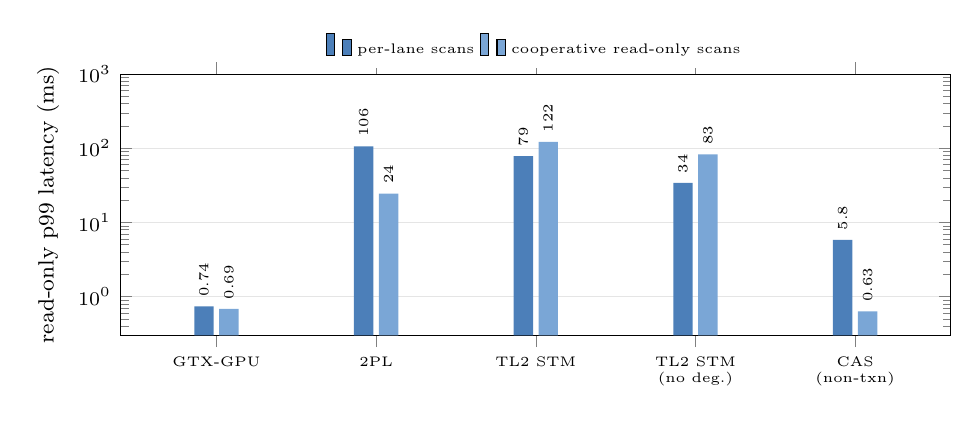
\begin{tikzpicture}
\begin{axis}[
  width=\columnwidth, height=4.9cm, ybar, bar width=7pt, ymode=log, log origin=infty,
  ymin=0.3, ymax=1000, symbolic x coords={GTX,2PL,TL2,TL2nd,CAS}, xtick=data,
  xticklabels={\sys{}, 2PL, TL2 STM, {TL2 STM\\(no deg.)}, {CAS\\(non-txn)}},
  xticklabel style={align=center, font=\tiny}, tick label style={font=\scriptsize},
  ylabel={read-only p99 latency (ms)}, label style={font=\footnotesize},
  ymajorgrids, grid style={black!10}, enlarge x limits=0.15,
  legend style={font=\tiny, at={(0.5,1.02)}, anchor=south, legend columns=2, draw=none},
  nodes near coords, nodes near coords style={font=\tiny, rotate=90, anchor=west},
  point meta=explicit symbolic]
\addplot[fill=cGTX!80, draw=none] coordinates {(GTX,0.736)[0.74] (2PL,106.0)[106] (TL2,78.5)[79] (TL2nd,34.1)[34] (CAS,5.80)[5.8]};
\addlegendentry{per-lane scans}
\addplot[fill=cCONS, draw=none] coordinates {(GTX,0.685)[0.69] (2PL,24.5)[24] (TL2,121.8)[122] (TL2nd,83.0)[83] (CAS,0.632)[0.63]};
\addlegendentry{cooperative read-only scans}
\end{axis}
\end{tikzpicture}
\caption{Read-only transaction p99 latency, R-MAT with 90\% readers, $K{=}4$. \sys{} scans cooperatively in both
bars; the modes refer to the baselines.}
\label{fig:latency}
\end{figure}

\subsection{Serializable transactions}
At full size ($|V|{=}2^{20}$, read-write $K{=}4$ with 20\% read-only transactions), SER \sys{} is 2,128$\times$ and
420$\times$ faster than 2PL and TL2 on Zipf, and 652$\times$ faster than TL2 on a 50\% hub, where 2PL does not finish.
The degree-free STM is faster in these write-dominated mixes: \sys{} reaches 0.64$\times$ (Zipf), 0.75$\times$ (hub)
and 0.80$\times$ (uniform) of it. On uniform read-write, SER \sys{} is 0.49$\times$ of 2PL and 1.61$\times$ of TL2.
SER costs \sys{} 6--15\% relative to SI. All systems pass C1--C5 in the checked SER runs.

\subsection{Real graphs}
\label{sec:snap}
Four SNAP graphs are replayed as sliding-window streams: edges are shuffled with a fixed seed, the first 80\% form
the initial graph, inserts take unseen tail edges, deletes remove the oldest initial edges, and reads and scans target
random edges. \sys{} is bulk-loaded with each vertex's first generation sized to its degree; the baselines are pre-sized
for the initial graph and all future inserts (Table~\ref{tab:snap}).

\begin{table}[t]
\caption{SNAP sliding-window streams: speedup of \sys{} (committed transactions/s).}
\label{tab:snap}
\footnotesize
\setlength{\tabcolsep}{2.5pt}
\begin{tabular}{@{}P{2.25cm}P{1.75cm}rrr@{}}
\toprule
Graph ($|V|$, $|E|$, max deg.) & Stream & 2PL & TL2 & TL2 no-deg \\
\midrule
wiki-Talk (2.4M, 5.0M, 100K) & ins $K{=}1$ & 34$\times$ & 96$\times$ & 1.01 \\
 & churn $K{=}4$ & 1,103$\times$ & 395$\times$ & 1.02 \\
 & SER rw $K{=}4$ & 533$\times$ & 301$\times$ & 1.05 \\
 & 90\% readers & 196$\times$ & 30$\times$ & 20.6$\times$ \\
soc-pokec (1.6M, 30.6M, 8.8K) & churn $K{=}4$ & 1.01 & 4.78 & 0.73 \\
 & 90\% readers & 1.19 & 6.80 & 5.39 \\
cit-Patents (3.8M, 16.5M, 770) & churn $K{=}4$ & 0.73 & 2.01 & 0.71 \\
 & 90\% readers & 1.12 & 2.41 & 1.91 \\
roadNet-CA (2.0M, 5.5M, 12) & churn $K{=}4$ & 0.70 & 1.72 & 0.76 \\
 & 90\% readers & 0.84 & 1.38 & 1.06 \\
\bottomrule
\end{tabular}
\end{table}

wiki-Talk, with a 100K-degree hub, behaves like the synthetic hub cells. Graphs without extreme hubs (roadNet-CA,
cit-Patents) behave like the uniform cells: \sys{} is 0.66--0.84$\times$ of 2PL on update and SER streams, and it still
beats TL2 with a degree word except on $K{=}1$ churn. soc-pokec sits between the two and wins as readers grow.

\subsection{Comparison with GPMA+}
GPMA+ applies a sorted batch as one unit and offers no multi-edge transactions or concurrent readers. We fed it the
exact $K{=}1$ streams used for \sys{}, and report the faster of the upstream build and our Windows port
(Table~\ref{tab:gpma}). \sys{} commits every operation as its own transaction. It is 6.6--15.2$\times$ faster on
streams where GPMA+'s final graph verifies correct, with outliers of 51$\times$ (wiki-Talk inserts) and 296$\times$
(roadNet-CA inserts, where GPMA+ hits multi-second rebalances). On synthetic hub and churn streams, GPMA+ loses
intra-batch operation order (a batch can insert and delete the same edge) and its final graph is wrong; there \sys{} is
5.8--9.5$\times$ faster.

\begin{table}[t]
\caption{GPMA+ vs.\ \sys{} on identical $K{=}1$ streams (effective edges/s; 65,536-edge batches unless noted).}
\label{tab:gpma}
\footnotesize
\setlength{\tabcolsep}{3pt}
\begin{tabular}{@{}lrrcr@{}}
\toprule
Stream & GPMA+ ms & \sys{} ms & GPMA+ verify & Speedup \\
\midrule
uniform insert & 44.4 & 3.90 & pass & 11.4$\times$ \\
uniform insert (524K batch) & 34.8 & 3.90 & pass & 8.9$\times$ \\
uniform churn & 28.6 & 4.40 & fail & 6.5$\times$ \\
50\% hub insert & 28.2 & 2.96 & fail & 9.5$\times$ \\
wiki-Talk insert & 61.4 & 1.19 & pass & 51.5$\times$ \\
soc-pokec insert / churn & 117.2 / 72.9 & 7.74 / 8.60 & pass & 15.2 / 8.5$\times$ \\
cit-Patents insert / churn & 101.5 / 60.1 & 8.22 / 9.15 & pass & 12.3 / 6.6$\times$ \\
roadNet-CA insert / churn & 1,137 / 34.6 & 3.84 / 4.20 & pass & 296 / 8.2$\times$ \\
\bottomrule
\end{tabular}
\end{table}

\paragraph{Batch size.} With one kernel launch per batch (GPMA+'s unit of atomicity, so \sys{} gets no cross-batch
overlap) on 4M uniform churn operations, \sys{} takes 225~ms at $2^{10}$-edge batches, where launches dominate, and is
flat at 18--21~ms from $2^{16}$ upwards. GPMA+ amortizes its sort and rebalance only at very large batches. The speedup
falls from 14--16$\times$ (batches $\le 2^{12}$) to 4.2$\times$ at $2^{20}$ and 1.8$\times$ at $2^{22}$. GPMA+'s final
state is wrong at every batch size on this stream.

\subsection{Ablation and design hypotheses}
\label{sec:ablation}
Each GPU mechanism was stated with a falsification criterion before measurement (Table~\ref{tab:hyp}). The M1 and M3
measurements are from the 2026-09 campaign.

\textbf{M1: cooperative reservation} (\code{gtx} vs \code{gtx-dst-only}, identical except \code{coop}). The
hypothesis was a $\ge$10\% gain on hub workloads. Measured gains were +8.6\% and +11.0\% on 50\% hub at $K{=}1$ and
$K{=}8$, +6.0\% and +5.8\% on 100\% hub, and +3.4\% on uniform $K{=}8$. Three of the four hub cells are below
threshold, so M1 is \emph{falsified as a primary mechanism}. Same-address RMWs on Ada's L2 are not the hub bottleneck.
It is kept as a small win that was never negative.

\textbf{M1b: destination-precise conflicts} (\code{gtx} vs \code{gtx-cons}). This is \emph{supported}.
Figure~\ref{fig:aborts} shows the abort ratio: chain-granularity aborts grow with $K$ to 42\% (uniform) and 38\% (hub)
at $K{=}32$, while destination-precise detection has zero aborts on uniform and 23\% on the hub (true conflicts).
In the 2026-11 campaign, throughput improves $\times$1.09 at uniform $K{=}8$, and $\times$1.67 (uniform) and
$\times$1.30 (hub) at $K{=}32$ over the conservative port.

\textbf{M3: epoch commit groups.} \emph{Not falsified.} Commit takes 9.6\% (4M-edge initial graph) to 15.5\% (empty
graph) of the lane-cycle profile for uniform $K{=}1$ inserts, below the 25\% threshold, and all histories pass.

Two micro-optimizations were also falsified: padding hot counters onto separate cache lines (no gain, reverted), and
relaxed versus acq\_rel reservation RMW (no measurable difference, so the fence required by D8 is free here).

\begin{figure}[t]
\centering
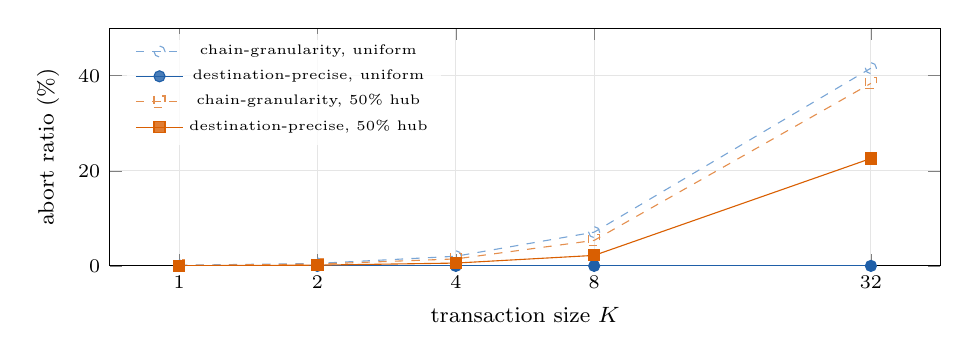
\begin{tikzpicture}
\begin{axis}[
  width=\columnwidth, height=4.6cm,
  xmode=log, log basis x=2, xtick={1,2,4,8,32}, xticklabels={1,2,4,8,32},
  ymin=0, ymax=50, grid=major, grid style={black!10},
  xlabel={transaction size $K$}, ylabel={abort ratio (\%)},
  tick label style={font=\scriptsize}, label style={font=\footnotesize},
  legend style={font=\tiny, at={(0.02,0.98)}, anchor=north west, draw=none, fill=white, fill opacity=0.8, text opacity=1}]
\addplot[cCONS, mark=o, dashed] coordinates {(1,0.132)(2,0.523)(4,2.03)(8,7.10)(32,41.6)}; \addlegendentry{chain-granularity, uniform}
\addplot[cGTX, mark=*] coordinates {(1,0)(2,0)(4,0)(8,0)(32,0)}; \addlegendentry{destination-precise, uniform}
\addplot[cTPL!70, mark=square, dashed] coordinates {(1,0.0901)(2,0.382)(4,1.47)(8,5.37)(32,38.4)}; \addlegendentry{chain-granularity, 50\% hub}
\addplot[cTPL, mark=square*] coordinates {(1,0.0384)(2,0.156)(4,0.595)(8,2.21)(32,22.6)}; \addlegendentry{destination-precise, 50\% hub}
\end{axis}
\end{tikzpicture}
\caption{Abort ratio under GTX's chain-granularity rule (GTX-conservative) and \sys{}'s destination-precise
validate-then-CAS (insert-only workloads, 2026-11).}
\label{fig:aborts}
\end{figure}

\begin{table}[t]
\caption{Design hypotheses and outcomes.}
\label{tab:hyp}
\footnotesize
\setlength{\tabcolsep}{2.5pt}
\begin{tabular}{@{}P{2.3cm}P{3.2cm}P{2.0cm}@{}}
\toprule
Method & Falsified if & Outcome \\
\midrule
M1 cooperative reservation & $<$10\% gain on hub, $K\in\{1,8\}$ & falsified (+3.4--11\%) \\
M1b destination-precise conflicts & $<$10\% gain at $K\ge 8$ or any checker failure & supported \\
M2 multiple reservation regions & $<$10\% gain on 100\% hub & not built (ranked low after M1) \\
M3 epoch commit groups & commit $>$25\% of cycles, or C1--C5 failure & not falsified (9.6--15.5\%) \\
M4 merging + block reuse & P1 bytes, P2 time, P3 gate + mutations & falsified (P1, P2); P3 fails as registered \\
M5 quiescent compaction & Q1 bounded, Q2 $\ge$0.85$\times$ e2e, Q3 gate + mutations & Q1 met on uniform and Zipf; fails on identical-edge-1024 (live graph grows) and on R-MAT with the tuned policy (never triggers); Q2 passes (near-empty window; 0.70--0.81$\times$ vs a 3$\times$ arena); Q3 fails as registered ($F{-}1$ not observable) \\
\bottomrule
\end{tabular}
\end{table}

\subsection{Memory and version reclamation}
\label{sec:memory}
\paragraph{Where the bytes are.} Memory was measured before any redesign (\code{--membreak}). Unwritten capacity in
each vertex's newest generation, a result of the $8\times$ growth ladder and \code{minCap}${=}8$, is 43--61\% of all
bytes. Chain heads scale with capacity. Reclaimable garbage (voided, aborted, dead and DEL versions) is only 0\% of the
bytes on uniform inserts, 4\% on Zipf churn, 9\% on identical-edge-1024 and 14\% on identical-edge-64. Growing
generations by $2\times$ instead (\code{gtx-gs1}) cuts bytes by 20--55\% at $\le$1\% time on uniform and hot cells. It
costs 17--30\% on skewed live-insert workloads, because writers then walk more older generations (7$\to$18).

\paragraph{M4: merging, falsified.} Method~4 merges a vertex's generations into one and reuses freed blocks through
announcements, epoch-based reclamation and forwarding. It is proven (Appendix proof \S8), and gate sections F--H pass.
Against its registered criteria it is falsified on bytes (P1) and time (P2). On identical-edge-1024 it takes 749$\to$636~MB
but runs at $0.33\times$ of \sys{}, and \code{gtx-gs1} alone reaches 480~MB at no time cost. Each merge re-copies most
live versions: 84\% of linked versions are kept. P3 fails as registered, because one of the four registered
mutations is not observable on this GPU. M4 stays in the code, off by default.

\paragraph{M5: quiescent compaction.} Garbage is a small share of a full store, but it is the only part that grows
without bound. Every write leaves a version that is never reused, so with a fixed arena any stream eventually runs
out. Method~5 reclaims at kernel-launch boundaries, where no transaction or snapshot is open. It computes the graph
visible at the frontier $F$, discards the whole store and rebuilds it as a bulk-loaded state of that graph: one
generation per live vertex, every edge a committed insert with \code{cts}${=}1$. The proof (Appendix proof \S9,
Theorem~6) shows that the rebuilt store answers every later snapshot exactly like the old one would have. A trigger
runs before each launch. It compacts when the arena, head, block or descriptor space could not absorb $1.5\times$ the
largest per-launch growth seen so far. Large vertices (more than 4096 scanned slots) are split into 512-slot chunks and
rebuilt one thread block per vertex. This cut the Zipf pause from 27.4 to 10.0~ms.

\paragraph{Protocol.} The criteria were registered before the code was written
(\code{design/design.md} \S7). \textbf{Q1:} no OOM and no resource aborts over a run that writes $>3\times$ what the
arena holds, and a high-water over the last third of rounds $\le 1.10\times$ that over the middle third. \textbf{Q2:}
end-to-end throughput (kernels plus pauses) $\ge 0.85\times$ of \sys{} over the rounds \sys{} completes, on uniform,
Zipf and identical-edge-1024 churn. \textbf{Q3:} gate section I and three mutations. \textbf{Q4:} report the pauses.
Each run replays $2^{18}$ transactions per round ($K{=}4$, 50\% insert / 50\% FIFO delete) for 64 rounds on
$|V|{=}2^{20}$ with 4M initial edges and a 20M-slot arena. The reported policy (trigger, \code{growShift}${=}1$,
100\% rebuild slack) was chosen \emph{after} registration, from a sweep of seven policies on uniform and Zipf churn
(\code{results/m5/sweep.log}). The registered default (\code{growShift}${=}3$, no slack) is reported next to it.

\begin{table}[t]
\caption{M5 long runs, 64 rounds, 20M-slot arena (\code{results/m5/longrun.log}). ``Rounds'' is the number of rounds
completed before the first resource abort. One run per cell. Peak in MiB. Ratio: end-to-end throughput vs \sys{} with a $3\times$ arena (60M) over
the rounds that run completes (7, 22, 4 and 64 rounds; it also runs out on churn). Pause in ms (p50/max).}
\label{tab:m5}
\footnotesize
\setlength{\tabcolsep}{2.2pt}
\begin{tabular}{@{}lrrrrr@{}}
\toprule
Workload, system & Rounds & Peak & Last/mid & Ratio & Pause \\
\midrule
\multicolumn{6}{@{}l}{\emph{uniform churn}} \\
\quad \sys{} / \code{gtx-gs1} & 2 / 6 & 879 / 793 & -- & -- & -- \\
\quad M5 (policy) & 64 & 748 & 0.999 & 0.79 & 10.2/13.6 \\
\quad M5 (registered default) & 64 & 641 & 1.001 & 0.49 & 8.0/12.6 \\
\multicolumn{6}{@{}l}{\emph{Zipf churn}} \\
\quad \sys{} / \code{gtx-gs1} & 1 / 7 & 979 / 800 & -- & -- & -- \\
\quad M5 (policy) & 64 & 714 & 1.001 & 0.70 & 10.0/13.2 \\
\quad M5 (registered default) & 64 & 760 & 1.004 & 0.31 & 8.5/11.5 \\
\multicolumn{6}{@{}l}{\emph{identical-edge-1024 churn} (live graph grows)} \\
\quad \sys{} / \code{gtx-gs1} & 1 / 3 & 865 / 805 & -- & -- & -- \\
\quad M5 (policy) & 28 & 802 & -- & 0.81 & 9.4/16.4 \\
\quad M5 (policy), 40M arena & 64 & 1352 & 1.107 & -- & 12.6/20.7 \\
\multicolumn{6}{@{}l}{\emph{R-MAT, 90\% readers}} \\
\quad \sys{} & 13 & 760 & -- & -- & -- \\
\quad M5 (policy): never triggers & 64 & 804 & 1.108 & 1.00 & -- \\
\quad M5 (registered default) & 64 & 723 & 0.994 & 1.36 & 11.1/13.3 \\
\bottomrule
\end{tabular}
\end{table}

\paragraph{Results (Table~\ref{tab:m5}).}
\begin{itemize}
\item \textbf{Q1 is met on uniform and Zipf churn.} \sys{} and \code{gtx-gs1} exhaust the arena in rounds 1--7. M5
completes all 64 rounds (67M effective writes against a 20M-slot arena). It peaks at 714--748~MiB, and its
high-water is flat between the middle and the last third of the run.
\item \textbf{Q1 fails on identical-edge-1024 as registered.} In this stream inserts outnumber effective deletes, so
the \emph{live} graph grows by about 131K edges per round after round 15 (4.0M$\to$10.3M edges over 64 rounds). The live count is the same, to within tens of edges, under every compaction schedule, so the growth
comes from the stream and not from a leak. No reclaimer can keep
that within a fixed arena. M5 runs out at round 28 with 5.7M live edges. With a 40M arena it completes 64 rounds, and
its memory follows the live graph at about 130 bytes per live edge (last/mid 1.107, just above the 1.10 bound).
M5 bounds memory by the live graph, not by a constant.
\item \textbf{Q2 passes as registered, but the window is nearly empty.} \sys{} completes only 1--2 rounds before it
runs out, and M5 does not need to compact in them (ratio 0.91--1.02). The useful comparison is against \sys{} with a $3\times$ arena, over
that run's clean rounds (7, 22 and 4). There M5 reaches $0.79\times$ on uniform, $0.70\times$ on Zipf and
$0.81\times$ on identical-edge-1024 churn. The registered default policy compacts nearly every round and reaches only
$0.31$--$0.49\times$.
\item \textbf{Read-heavy streams gain.} On R-MAT with 90\% scanning readers, version chains slow every reader: a
round of \sys{} grows from 5.5 to 12.2~ms over 64 rounds. The registered default compacts 5 times and holds rounds at
5.7~ms, $1.36\times$ the end-to-end throughput of the large-arena run. With \code{growShift}${=}1$ the arena never
fills, so the chosen policy never compacts there, and its high-water keeps rising (last/mid 1.108). The policy is
workload-dependent.
\item \textbf{Q3 fails as registered.} Gate section I runs multi-round histories with compaction between rounds in SI and SER and in
every writer and scan mode. It covers three kernel variants: the default hybrid kernels, the chunked path forced on
every vertex, and the first warp-per-vertex kernels. Every round is history-checked from the state before
compaction, and all 110 cases pass. The checker rejects two of the three registered mutations (drop one live edge
per vertex, keep invalidated versions). The third, compacting at $F{-}1$, is not observable at a launch boundary: the
last epoch normally holds no committed writer, so visibility at $F{-}1$ equals visibility at $F$ (Appendix proof
\S9). It is reported as informational. A substitute registered after the fact, a stale frontier $F/2$, is rejected.
\item \textbf{Q4.} Pauses are 8--12~ms at the median and at most 21~ms, about 2.5~ms per million live edges. A
compaction is stop-the-world: no transaction runs during it.
\end{itemize}

\paragraph{Limits.} M5 needs launch boundaries. A single kernel that never returns still grows, and a launch whose
growth exceeds the margin can still exhaust the arena inside the kernel. It requires M4 to be off. The policy was
tuned after registration on two of the four workloads.

\subsection{Where \sys{} loses}
\label{sec:losses}
Table~\ref{tab:losses} lists every scenario in which \sys{} is slower. The uncontended gap to 2PL is not in the write
path: removing the entire versioned install (not a valid execution) still leaves \sys{} 16--21\% behind 2PL on
uniform inserts. The transaction skeleton alone (descriptors, epochs, the attempt loop and the advancer) costs more
than 2PL's whole run.

\begin{table}[t]
\caption{Scenarios where \sys{} is slower (\sys{} / baseline throughput, 2026-11).}
\label{tab:losses}
\footnotesize
\setlength{\tabcolsep}{2.5pt}
\begin{tabular}{@{}P{2.6cm}P{1.1cm}P{4.0cm}@{}}
\toprule
Scenario & Ratio & Reason \\
\midrule
uniform, small transactions, vs 2PL & 0.37--0.56 & transaction skeleton (descriptors, epochs, attempt loop); uncontended locks are cheap \\
real graphs without hubs vs 2PL & 0.66--0.84 & same cause (roadNet-CA, cit-Patents) \\
write-heavy work vs TL2 without degree word & 0.58--0.87 & that STM cannot serve degree queries and is 5.4--20.6$\times$ slower once scanning readers arrive \\
almost any scenario vs non-txn CAS & 0.07--0.71 & CAS offers no atomicity or snapshots \\
memory vs pre-sized hash tables & 3--19$\times$ & versions, chain heads and layout (\S\ref{sec:memory}) \\
long streams with compaction & 0.70--0.81 & stop-the-world compaction pauses (\S\ref{sec:memory}) \\
\bottomrule
\end{tabular}
\end{table}

\subsection{Threats to validity}
The baselines' hash tables are pre-sized and never grow, which favours them. Scans were compared in both per-lane
and cooperative modes, and the better mode of each baseline is reported. DNF lower bounds assume the baseline would
have finished at the timeout. The 1.4--2.7$\times$ timing shift between campaigns was not isolated. The proof is a
hand proof, and one M4 hazard is covered by the proof only. The \code{gtx-m4} performance rows predate the
truncated-merge fix, which the gate covers. faimGraph was not run: a driver on identical streams exists, but
building the third-party code was not permitted, and Hornet, SlabGraph and LPMA are Linux-only or unavailable. The M5
compaction policy was chosen after a sweep run once the criteria had been registered (\S\ref{sec:memory}). All
experiments use one laptop GPU under WDDM.

%% ===================================================================================================================
\section{Limitations and Future Work}
\label{sec:limits}
\begin{enumerate}
\item \textbf{Reclamation inside a kernel.} M5 bounds memory only for workloads that return to the host between
launches. A single kernel that never returns still grows until the arena is exhausted, and a round that grows by more
than the projected margin can exhaust the arena before the next boundary. Online reclamation needs announcement-based
protection as in M4, but without M4's re-copying cost.
\item \textbf{Compaction pauses.} Compaction is stop-the-world. Overlapping it with a running kernel, or compacting
only the vertices that changed, would remove most of the pause.
\item \textbf{The memory floor}: smaller versions (split hot and cold delta fields) and fewer chain heads.
\item \textbf{The uncontended gap}: cheaper per-attempt bookkeeping; the write path is not the cause.
\item \textbf{Broader comparisons}: faimGraph (driver written, not built), Hornet, SlabGraph and LPMA on a Linux host.
\item \textbf{Out of scope}: vertex insertion and deletion, durability, and multiple reservation regions (M2).
\end{enumerate}

%% ===================================================================================================================
\section{Conclusion}
\sys{} shows that GTX's architecture (versioned edge deltas, destination-indexed delta chains, lazily resolved
descriptors and epoch group commit) transfers to the GPU, provided four parts are redesigned for SIMT execution:
conflict detection must validate and install on the same observed head, blocks must grow by generations instead of
copying, commit registration must be a single wait-free RMW, and serializable validation must follow the epoch. The
result offers multi-edge transactions and non-blocking snapshot readers, which no existing GPU dynamic-graph structure
provides. It outperforms lock-based and word-STM synchronization by one to four orders of magnitude where
synchronization is hard, and it pays a bounded, measured cost where it is easy. Memory, the main gap of the first
version, is bounded by quiescent compaction for workloads that reach kernel boundaries and whose live graph fits
the arena, at a measured throughput cost.
A history checker that validates every operation, together with a paper proof, was essential: between them they found
eight protocol defects, two of which no test could observe. We consider both a necessary part of any claim about GPU
transaction protocols.

\bibliographystyle{ACM-Reference-Format}
\bibliography{refs}

\appendix
\section{Reproducing the Results}
All code, raw data and scripts are in the \code{gtx-gpu-research} repository.
\begin{itemize}
\item Correctness gate (sections A--I): \code{build.bat test\_gtx \&\& bin\textbackslash test\_gtx.exe full}.
\item Benchmarks: \code{build.bat bench}; \code{python scripts/campaign\_v2.py}; tables by
\code{python scripts/report\_tables\_v2.py} (\code{results/v2/}).
\item Long runs and compaction: \code{python scripts/sweep\_m5.py}, \code{python scripts/longrun\_m5.py}
(\code{results/m5/}).
\item GPMA+: \code{baselines/gpma/build\_gpma.bat}; \code{python scripts/run\_gpma.py}.
\item Source map: \code{src/gtxg.cuh} (engine, M4, M5), \code{src/baselines.cuh} (2PL, TL2, CAS),
\code{src/checker.hpp} (C1--C5), \code{src/harness.hpp} (runs, long runs), \code{src/workload.hpp} (generator),
\code{src/bench.cu}, \code{src/test\_gtx.cu}; proof in \code{design/proof.md}.
\end{itemize}

\end{document}
